The reference-predication trade-off hypothesis was tested in four behavioural web-based experiments employing different dependent measures. The crucial manipulation in all experiments was the varying position of the critical noun - it appeared either in the subject (e.g., “That N is ADJ” or “That ADJ N is N2”) or in the predicate (“That’s a ADJ N” or “That N2 is a ADJ N”) of the sentences presented in the experiments. These sentences described a depicted object which appeared in visual context. 

These objects were sampled from five different basic-level categories: dogs, birds, flowers, trees and fish \parencite{rosch1976}. Within each basic-level category, at least two subordinate categories were chosen which exhibit a rather high or rather low amount of the feature described by the gradable adjectives under investigation - that is, those subordinate categories were chosen which people expect to be rather large or rather small representatives of their basic-level categories (s. table \ref{tab:stimuli}). For example, for the \textit{dog}-category, the large-subordinate category \textit{Great Danes} and the small-subordinate category \textit{pugs} were chosen. As shown by \textcite{tessler2017warm}, when encountering representatives of such categories described by the adjective consistent with participants’ prior expectations about the degree of feature-under-discussion, people are a priori more likely to infer the basic-level comparison class than the subordinate comparison class. For example, when encountering the sentence “It’s big” said of a Great Dane (a large-subordinate category for the basic-level category dogs), humans are more likely to infer that the Great Dane is big relative to other dogs in general, than big relative to other Great Danes.  
Following the design of \textcite{tessler2017warm} in these experiments allows to test the effect of syntactic position of the noun on how strong the noun is taken to constrain the comparison class: The reference-predication trade-off hypothesis predicts that nouns in the predicate position constrain the comparison class more strongly than in the subject position, such that a priori using the basic-level noun in predicate position is more felicitous in order to describe a normal-sized large-subordinate object (e.g., a Great Dane) than using a subordinate-label of the object in predicate position. Both nouns would be felicitous in the subject position. Furthermore, encountering a subordinate label in the predicate position, should signal a more extreme feature value than the basic-level label.

\begin{table}[t]
	\small{
		\begin{center}
			\caption{Experimental items: each basic-level context had two potential targets from an either saliently small or saliently big subordinate category within the basic-level class. Items marked with * were used only in Expt. 2., items marked with $^{+}$ were used in all experiments including Expt. 4}
			\label{tab:stimuli}
			\vskip 0.12in
			\fontsize{10}{11}\selectfont
			\begin{tabularx}{\textwidth}{XXX}
				\hline
				Basic-level category & Smaller referent & Bigger referent\\
				\hline
				Dogs$^+$ & Pug$^+$ & Great Dane$^+$ \\
				Dogs$^+$ & Chihuahua$^+$ & Doberman$^+$\\
				Birds$^+$ & Hummingbird$^+$ & Eagle$^+$  \\
				Fish & Goldfish & Swordfish \\
				Flowers$^+$ & Dandelion$^+$ & Sunflower$^+$\\
				Trees$^+$ & Bonsai$^+$ & Redwood$^+$\\
				Birds* & Sparrow* & Goose* \\
				Birds* & Canary* & Swan* \\
				Fish* & Clownfish* & Tuna* \\
				Flowers* & Daisy* & Peony* \\
				\hline     
			\end{tabularx}
		\end{center}
	}
\end{table}

In all experiments, the referents were described by the adjective matching prior feature-degree expectations; for instance, Great Danes and sunflowers were always described as \textit{big}, and pugs or daisies as \textit{small}. 

\begin{figure*}[t]
	\begin{center}
		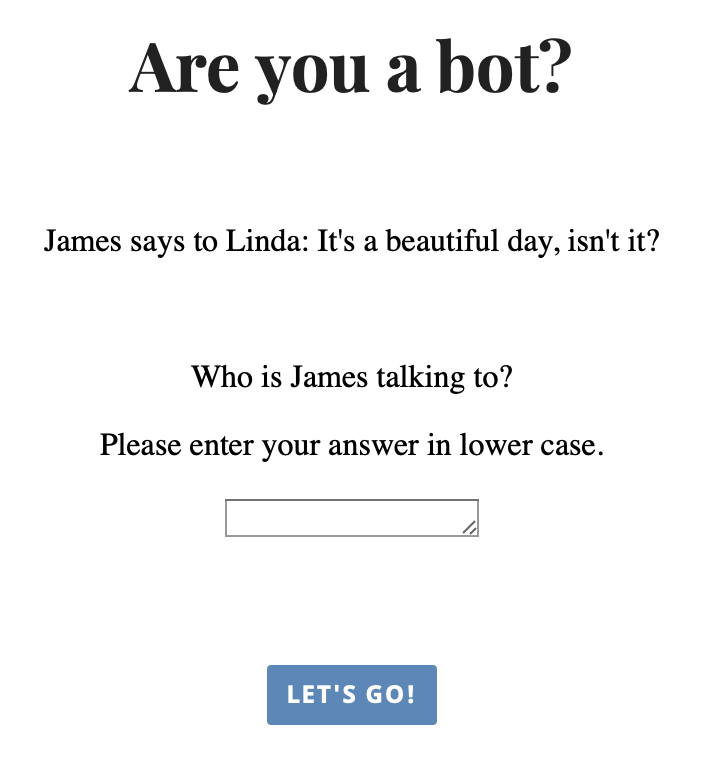
\includegraphics[width=0.5\linewidth]{captcha.png}
	\end{center}
	\caption{Example view of the bot check trial: The speaker James addresses the listener Linda.}
	\label{captcha}
\end{figure*}

The structure of all experiments was similar. First, participants completed a bot-check trial (Fig. \ref{captcha}): Participants read a sentence where a named speaker asked a named listener: “It’s a beautiful day, isn’t it?”. The speaker and listener names were sampled from lists of ten most popular male and female English names. For example, the sentences read: “John says to Mary: “It’s a beautiful day, isn’t?”; Who is John talking to?”.  Participants were asked to fill-in in lowercase who the listener is talking to. Participants were provided feedback and had maximally three attempts to fill-in the correct name. They were only allowed to proceed, if they successfully completed the bot check. Then, participants read instructions and completed practice trials, before completing main trials. After the main trials, they completed a socio-demographic post-test questionnaire, where they were asked to indicate their native language and optionally provide further information. 
For all experiments, participants were recruited via the crowd-sourcing platform Amazon’s Mechanical Turk; only participants with IP addresses in the United States and work approval rating of at least 95\% were permitted to participate. Participants were restrained from taking part in multiple experiments of this series.  

The first experiment (E1, Sentence Rating Experiment) was a sentence rating experiment, wherein participants had to rate two sentences which differed in the position of the noun (subject-N ~vs.~ predicate N) and the specificity of the noun, as describing an object in context. 
In the second experiment (E2, Noun Production Experiment), participants had to fill-in the missing noun of a sentence describing the size of a referent in context. The position of the missing noun was varied. 
In the third experiment (E3, Comparison Class Inference Experiment), participants provided the inferred comparison classes via a free-production paraphrase, given sentences which varied by the noun category and its position, as describing a referent in different contexts. 
Finally, the fourth experiment (E4, Direct Modification Experiment) gathered inferred comparison classes in a paradigm akin to E3, but from sentences wherein the critical noun appearing in subject or predicate position was always syntactically modified by the adjective. 
All experimental materials can be found under \texttt{https://github.com/polina-tsvilodub/refpred}, and  the preregistrations can be found under \texttt{tinyurl.com/yb5ogj5g}. \pt{preliminary link} All experiments were realized using the \_magpie - framework \parencite{magpie}. 
All experiments can be viewed under \texttt{tinyurl.com/yb5ogj5g}. \pt{also preliminary}

\section{Experiment 1: Sentence Rating Experiment}

%Results: main, by-participant / by-item variation, different exclusion criteria 

The aim of the sentence rating experiment was to investigate whether participants prefer one syntactic frame over the other, given two truth-conditionally equivalent sentences, depending on the nouns. The type of the noun and its syntactic position differed within-subjects.

\begin{figure*}[t]
	\begin{center}
		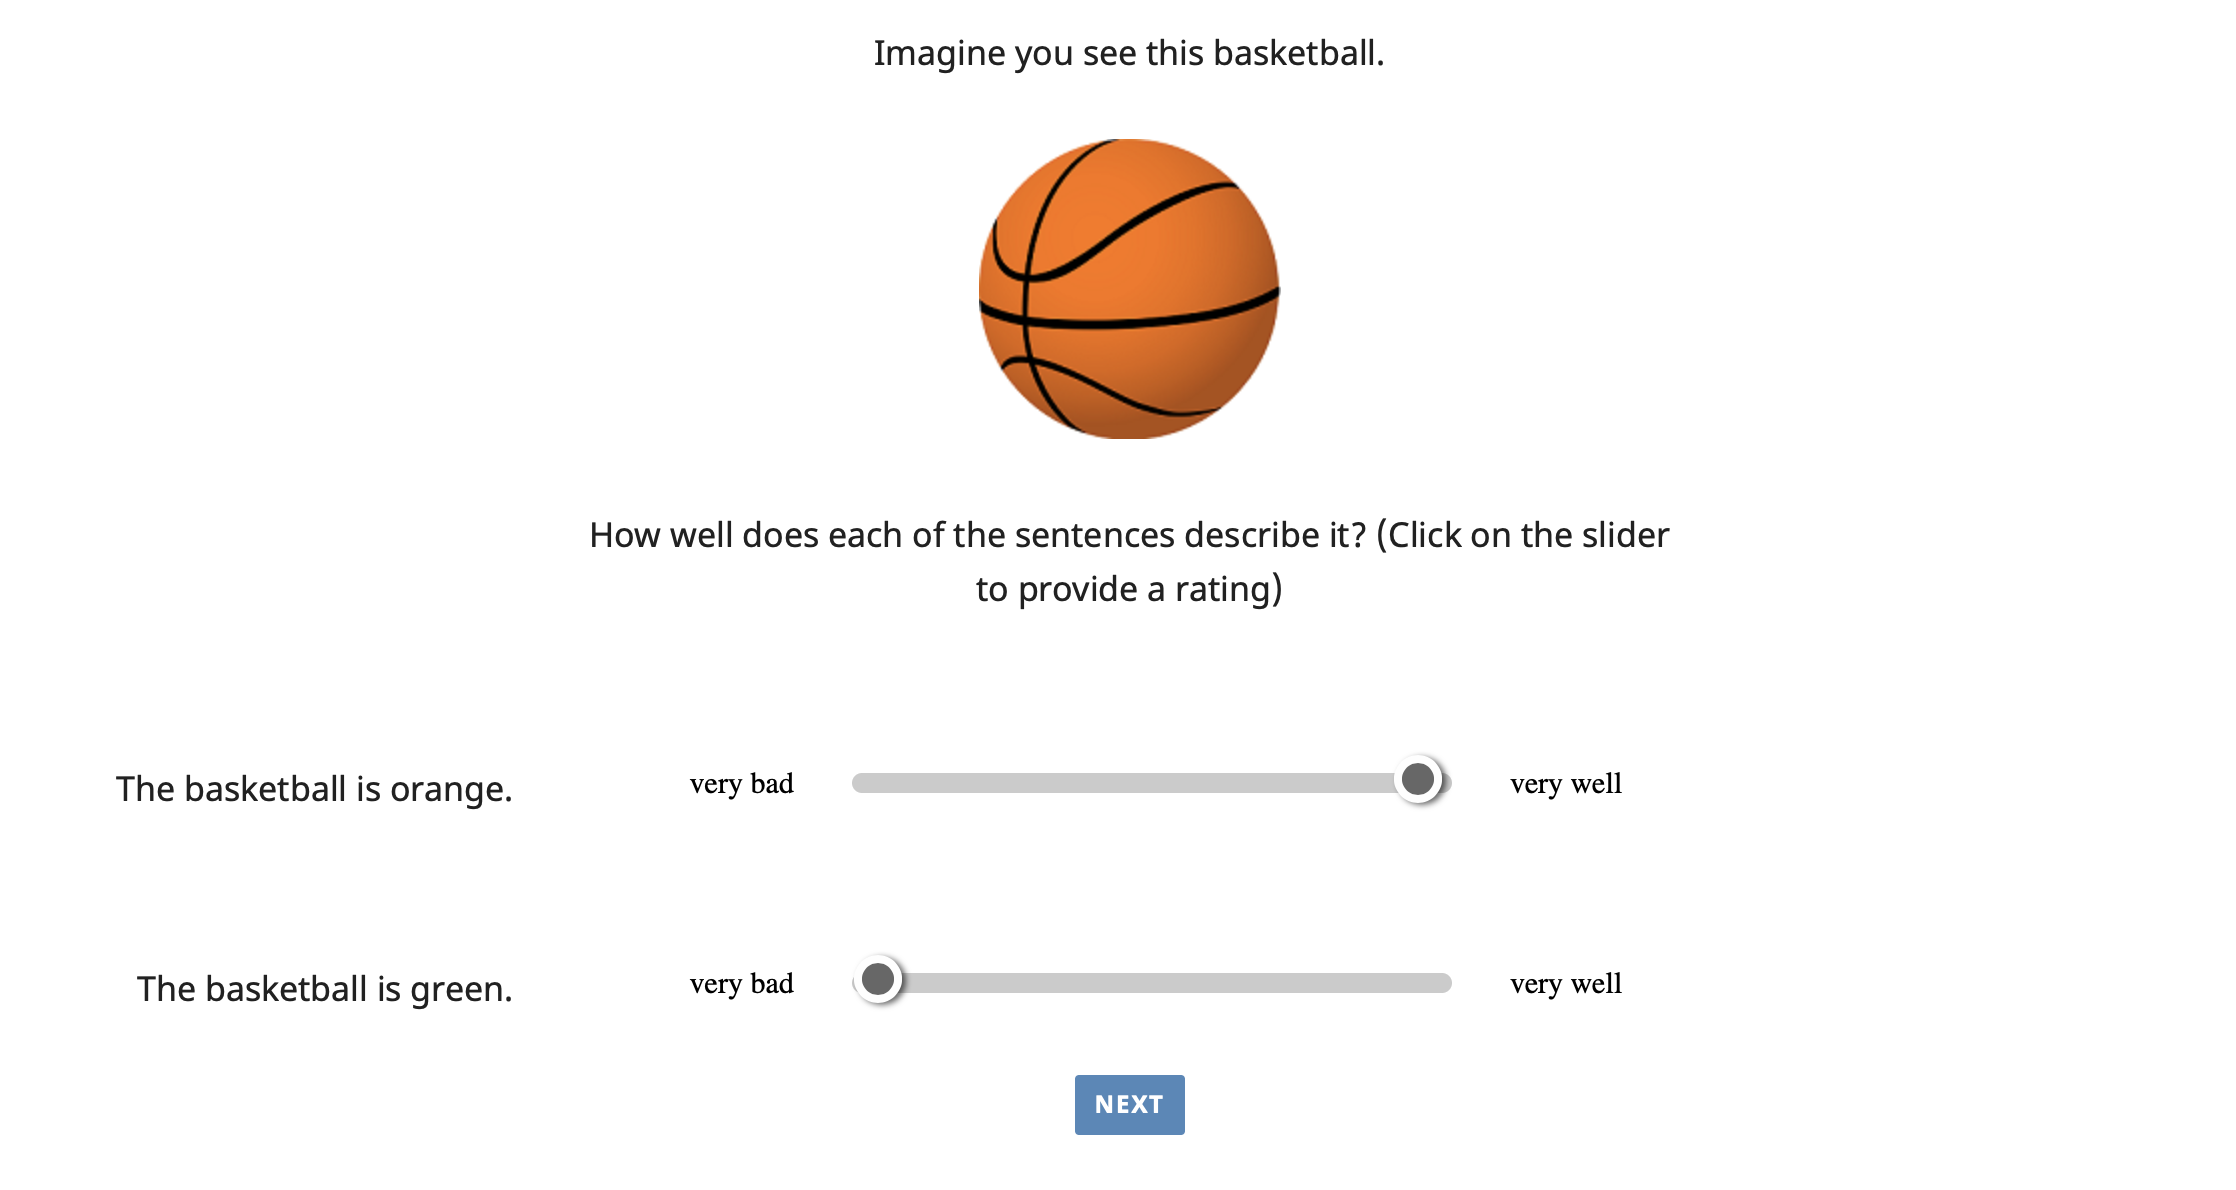
\includegraphics[width=0.7\linewidth]{warmup_basketball.png}
	\end{center}
	\caption{Example view of the sentence rating warm-up trial involving a basketball. \pt{Screenshots will be made more readable}}
	\label{warmup-basketball}
\end{figure*}
First, participants completed two warm-up trials to familiarize themselves with the slider rating procedure (Fig. \ref{warmup-basketball}). On one trial, participants read: “Imagine you see this basketball” above a picture of an orange basketball, and read below the question: “How well does each of the sentences describe it? (Please click on the slider to provide a rating)”. Two sentences appeared below: “The basketball is orange” and “The basketball is green”, to be rated on sliders ranging from “very bad” to “very well”. In the background, the ratings were mapped onto a scale ranging from 0 to 100. The slider was light gray, with a round handle appearing upon clicking on the slider track. The same sliders were used in the main trials. On the other warm-up trial, participants read: “Imagine you see this chair” above a picture of a purple chair. The sentences to be rated appearing below were: “The chair is yellow”, and “The chair is blue”. The order of the warm-up trials was randomized.    

\begin{figure*}[t]
	\begin{center}
		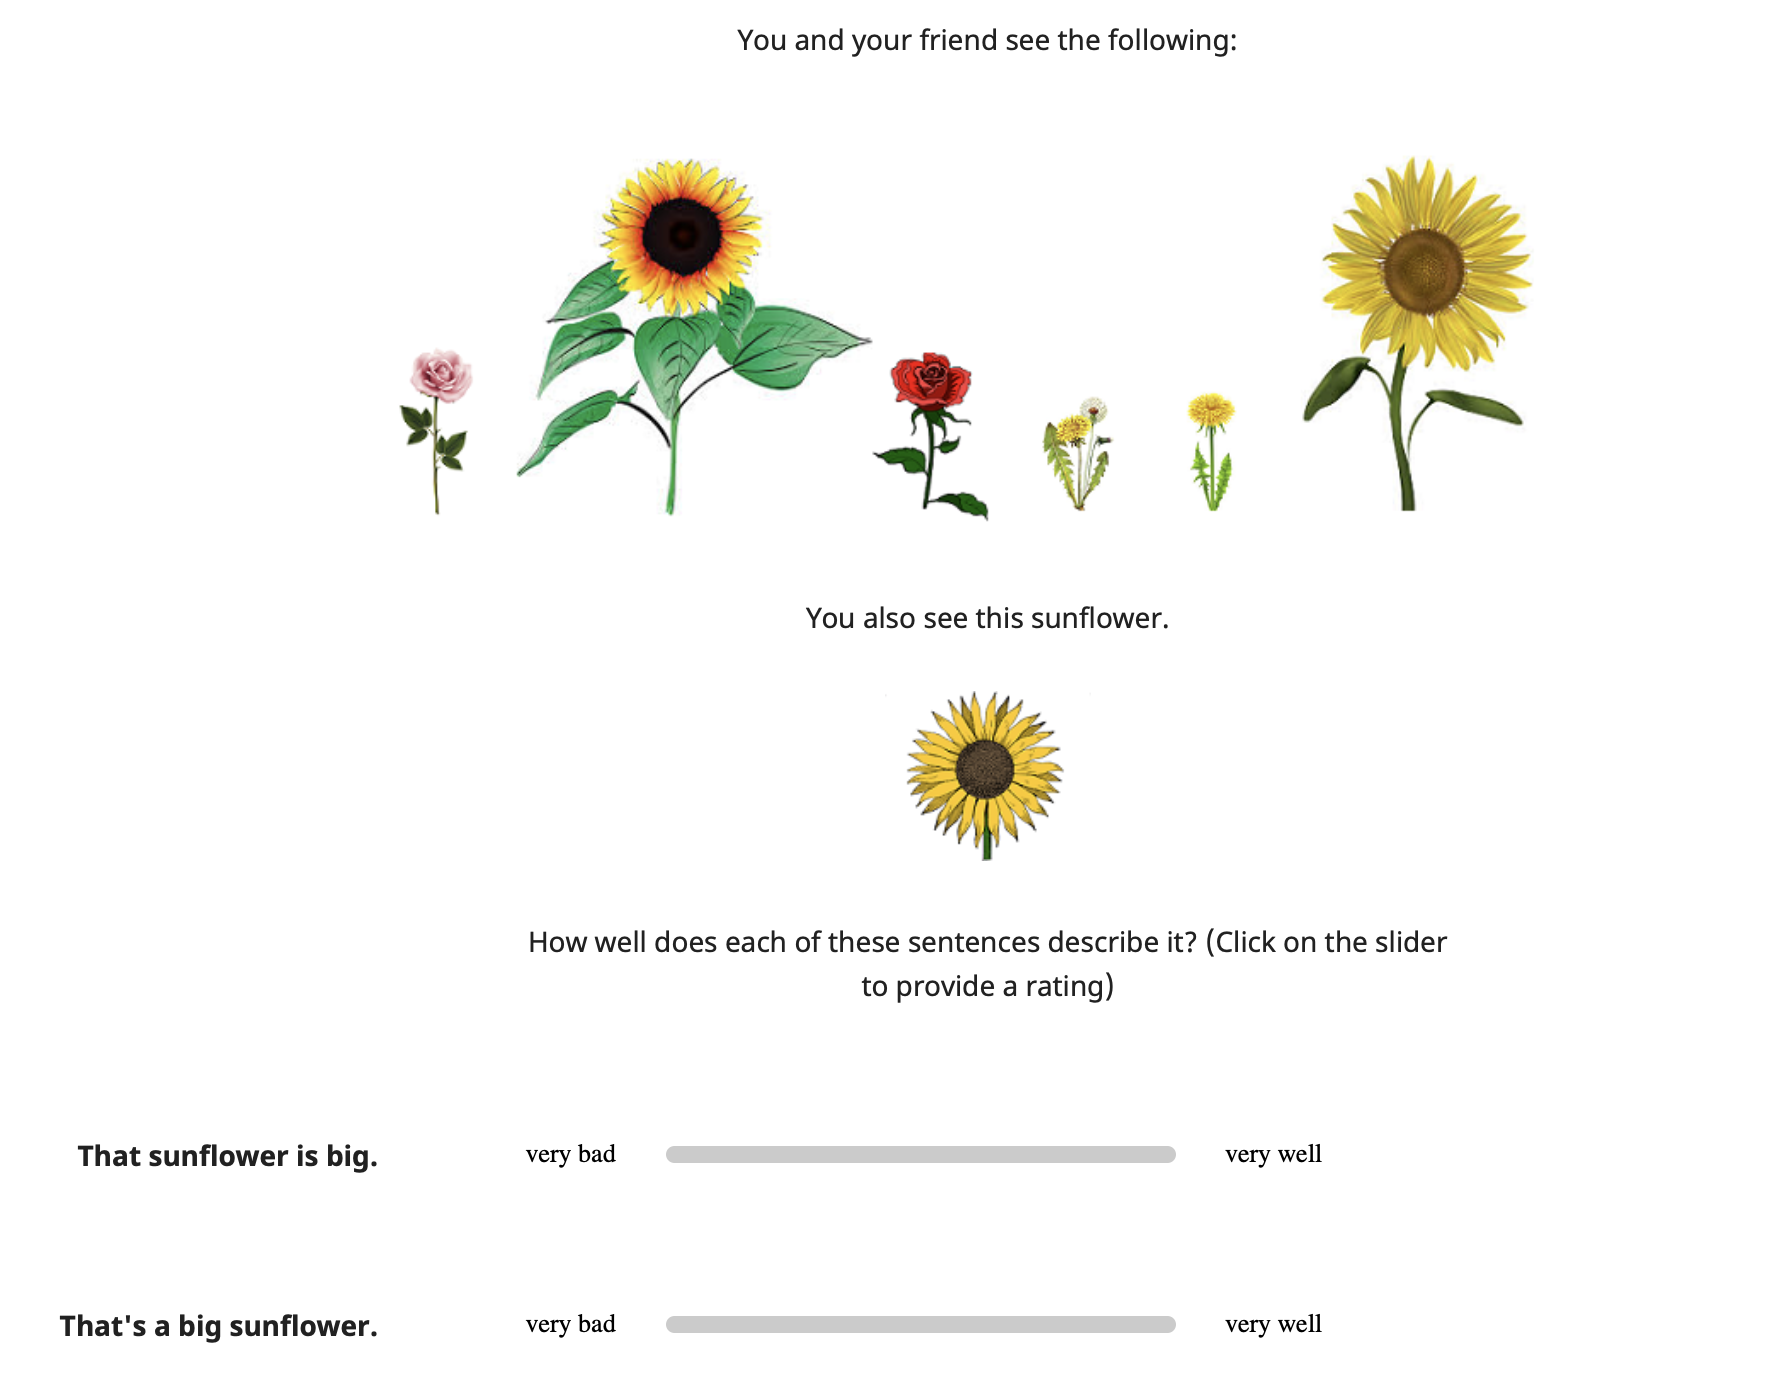
\includegraphics[width=0.7\linewidth]{main_rating_subN_big.png}
	\end{center}
	\caption{Example view of a sentence rating main trial: The critical noun is a subordinate target label of a large-subordinate category, appearing in the subject or predicate of the sentence.}
	\label{rating-main}
\end{figure*}
Then, participants completed six main trials (Fig. \ref{rating-main}). Participants read “You and your friend see the following:” above a basic-level context picture (e.g., a group of dogs). The picture consisted of six other members of the same basic-level category as the referent of the trial, including two other members of the same subordinate category as the referent. The six members consisted of two members of a large-subordinate, a medium-sized subordinate, and a small-subordinate category within the basic-level category each (e.g. the dog-context consists of two Great Danes, two poodles and two pugs). The context was used to set the overall reference comparison class for the targets. It also set the visual reference frame.
Below, they read the sentence “You also see this SUB\_N”, where SUB\_N was the subordinate label of the target referent, which appeared depicted below. The pictures depicted referents a little smaller than members of the same subordinate category in the context, such that the felicitous comparison class was pushed towards the basic level category of the target.
Below, the question about the critical sentences appeared: “How well does each of the sentences describe it? (Click on the slider to provide a rating)”. Then, the two critical sentences appeared left of the sliders one below the other. The sliders ranged from “very bad” to “very well”. On every trial, in one of the sentences the noun appeared in the subject (e.g. “That N is {big, small}”), in the other in the predicate position (“That’s a {big, small} N”). The order in which these syntactic conditions appeared was randomized between-subjects. 
On half of the trials, the noun was the basic-level target label (e.g., dog); on the other half it was the subordinate target label (e.g., Great Danes), balanced within-subjects. 
Participants saw each of the six possible contexts once, and for each context, one of the two possible targets (large-subordinate vs. small-subordinate category representatives) was sampled, balanced within-participants (Table \ref{tab:stimuli}). 

The reference-predication trade-off hypothesis predicts that sentences with a basic-level noun in the predicate position should receive a higher rating than sentences with a subordinate noun in predicate position, but there should be no difference in the ratings of the sentences with a basic-level compared to the subordinate noun in the subject position.  

\subsection{Participants}
113 participants were recruited and 33 were excluded for indicating a native language other than English, failing the practice trials or providing the same responses on every trial (see Appendix \ref{appendix}). The experiment took about 5 minutes and participants were compensated \$0.80. If partial data was missing from a participant, available data was used for analyses. 
\subsection{Results}
A Bayesian linear mixed-effects regression model was fit, predicting the sentence rating from the syntactic condition of the sentence (subject~vs.~predicate N), the noun type (basic-level~vs.~subordinate target label), their interaction and by-participant and by-target random intercepts and random effects of syntax, noun type and their interaction. \footnote{Model in \texttt{brm}-style syntax: \texttt{rating $\sim$ syntax * NP + (1 + syntax*NP | subject) + (1 + syntax*NP | target)}} 
An exploratory model including a main effect of syntactic condition order was also fit, revealing no effect of syntactic condition order, so the data was collapsed across the two conditions. Both predictors were deviation coded, coding both the subject-noun and the basic-level noun as 1 and the other levels as -1, respectively. 

Consistent with predictions, participants substantially dispreferred sentences with a subordinate noun in the predicate compared to the subordinate position, but no effect of syntax was found for the basic-level nouns, as indicated by the syntax X noun-type interaction ($\beta = \rlgetnum{expt1_brm.csv}{Rowname}{syntax:NP}{Estimate}{2}  [\rlgetnum{expt1_brm.csv}{Rowname}{syntax:NP}{l.95..CI}{2}, \rlgetnum{expt1_brm.csv}{Rowname}{syntax:NP}{u.95..CI}{2}]$). \footnote{All results report the mean and 95-\% Bayesian credible interval} 
Additionally, an overall preference for basic-level nouns ($\beta = \rlgetnum{expt1_brm.csv}{Rowname}{NP}{Estimate}{2} [\rlgetnum{expt1_brm.csv}{Rowname}{NP}{l.95..CI}{2},\rlgetnum{expt1_brm.csv}{Rowname}{NP}{u.95..CI}{2}] $) and the subject-noun syntactic structure ($\beta = \rlgetnum{expt1_brm.csv}{Rowname}{syntax}{Estimate}{2} [\rlgetnum{expt1_brm.csv}{Rowname}{syntax}{l.95..CI}{2}, \rlgetnum{expt1_brm.csv}{Rowname}{syntax}{u.95..CI}{2}] $) was found. Furthermore, a relatively high by-target variance revealed that some items received overall lower ratings, probably due to differing namability of the different items (by-target intercept: $\beta = \rlgetnum{expt1_random_brm.csv}{Rowname}{sd(Intercept)}{item.Estimate}{2} [\rlgetnum{expt1_random_brm.csv}{Rowname}{sd(Intercept)}{item.l.95..CI}{2}, \rlgetnum{expt1_random_brm.csv}{Rowname}{sd(Intercept)}{item.u.95..CI}{2}]$).
As expected, an exploratory analysis including a predictor of target size (small-subordinate vs. large-subordinate category) did not reveal any size-effects.

To sum up, the sentence rating experiment showed that participants are sensitive to the position and the type of the noun, dispreferring sentences where a noun that provided an infelicitous comparison appeared predicatively.  

\section{Experiment 2: Noun Production Experiment}    

%classification of responses
%results: main, by-participant / by-item, by-size  

The goal of the noun production experiment is to investigate whether in a free-production setting participants produce nouns of different categories, given different syntactic frames.  The noun of the critical sentences in the main trials appeared either in the subject position (e.g. in “That N is {big,small}“) or in the predicate position (e.g. in “That’s a {big,small} N”), manipulated between-subjects. 

In this experiment, participants completed two blocks, each consisting of three warm-up trials and three main trials. In the warm-up trials participants familiarize themselves with the subordinate categories used in the main trials. They see pictures of a member from a large-subordinate and a small-subordinate category within one of the basic-level categories used in the main trials (e.g. a Great Dane and a pug). Participants are prompted to provide labels for these pictures. Below they are prompted to provide a common label for both pictures (i.e. dogs). They are provided feedback for the labels and can proceed upon adjusting their labels to correct responses. The number of attempts participants needed until they filled-in the correct labels is recorded. In this experiment, four additional subordinate categories were used, which can be found in Table 1 marked with *. For each participant, six out of ten possible contexts are sampled. Three of these contexts and their corresponding targets appear in the first experimental block, and the other three in the second. The trial order within the warm-up block and the main block is randomized. 
On the main trials, participants read: “You see the following:” above a basic-level context picture, akin to the contexts used in experiment 1. Below, they read “You also see this one:” and see a picture of the target referent. Then they read: “You say to your friend:”, prompting them to fill-in the missing noun in the sentence: for the subject-noun condition, the template is “That\_\_ is {big, small}”, for the predicate-noun condition, the template to be completed is “That’s a {big, small} \_\_ “.  
The size of the target referent was balanced within-participants: on three trials, participants see referents from a small-subordinate category, and on three, they see referents from a large-subordinate category. For each context, participants see only one of the possible targets (e.g. the large or the small subordinate target).
Example trial view / example warm-up views
The reference-predication hypothesis predicts that participants should be less likely to produce subordinate target labels in the predicate compared to the subject position.

\subsection{Participants:}
242 participants were recruited, and 52 were recruited for indicating a native language other than English or for failing the warm-up trials. The exclusion criterion was taking more than four attempts on any warm-up trial to provide the correct label upon correction. The experiment took about 7 minutes and participants were compensated \$1.00. 
 
\subsection{Results:}
The responses provided by participants were categorized manually into basic-level or subordinate-level labels of the targets. X \% were superordinate referent labels (i.e. more general labels like animals) and were collapsed with basic-level labels. 16 (1.4\%) uncategorizable responses were excluded from analysis. 
A logistic generalized mixed-effects regression model was fit, regressing the response category (basic-level. vs subordinate target label) against the syntax of the sentence, random by-participant and by-referent intercepts and random by-referent slope effects of syntax. 
Consistent with predictions, a strong effect of syntactic position of the noun was found, indicating that participants were appreciably more likely to use basic-level labels in the predicative position (2.25 [0.74, 4.01]). 
Furthermore, different participants showed different sensitivity to the syntax, as indicated by… Additionally, by-referent variation was found, which could be attributed to differing namability of the targets. ….
An exploratory model including a main effect of referent size (large-subordinate vs. small-subordinate category) revealed that... 
 
 
\section{Experiment 3: Comparison Class Inference Experiment}
The two previous experiments support the reference-predication trade-off view, by showing that participants disprefer sentences like “That’s a big Great Dane” in order to describe a normal-sized Great Dane. The goal of this comparison class inference experiment was to measure comparison class inferences more directly, as influenced by the position of the critical noun in the sentence, the type of noun and the visual context of the sentence. All three factors are manipulated within-subjects.
When participants don’t have access to visually assessing the size of a referent and have to infer the comparison class from the sentence, they should be sensitive to linguistic cues like the sentence structure. According to the outlined hypothesis, they should be more likely to take the noun as a cue to the comparison class when the noun appeared in the predicate of that sentence, than when it appeared in the subject. When the noun appeared in the subject, comparison class inference can be driven by other pragmatic inference, e.g. from world knowledge and visual context. 
First, participants completed a comparison class paraphrase practice trial, akin to the paradigm employed in the main trials. Participants were told that on the main trials they will see a sentence containing a word that is relative, and their task will be to figure out what this word is relative to. They read an example task: “Speaker A: ‘The Empire State building is tall.’ What do you think speaker A meant?”. Below they saw a paraphrase template where they provided the inferred comparison class of the adjective tall: “The Empire State building is tall relative to other\_\_” (blank to be completed with the inferred comparison class). Participants were provided feedback on their response and had to correct it to one of the possible options among {buildings, skyscrapers, houses, constructions}. 
Then, participants completed two blocks consisting of labeling warm-up trials and main paraphrase trials. Three of the six basic-level categories used in this experiment (table 1) are sampled for the first block, with the respective subordinate category members appearing in the warm-up trials, the other three categories appear in the second block. These labeling warm-up trials are of the same kind as in Experiment 2. 
In this experiment, for the main trials there were basic-level and subordinate-level contexts for each possible referent. Basic-level contexts were identical to the contexts of respective categories in Experiment 1 and Experiment 2; the subordinate contexts consisted of six other representatives of the same subordinate category as the target referent. For example, the subordinate context for a Great Dane consisted of a picture of a group of six other Great Danes. Within each main trial block, there were six trials, wherein for each of the three sampled categories, one possible referent appeared in the corresponding basic-level context (e.g. for the category flowers, the sunflower appeared in basic-level flower context), and the other possible referent appeared in the corresponding subordinate context (i.e., then the daisy appeared in subordinate daisies-context). 
The referent was described by a critical sentence in which the noun could appear in the subject or in the predicate of the sentence. The noun could be either the basic-level (e.g. dog) or the subordinate label of the referent (e.g. Great Dane). Furthermore, a baseline condition with an anaphoric ‘one’ in the noun position was included, in order to measure the baseline influence of the visual context on comparison class inference (Goldberg and Michaelis, 2017). Crossing the visual context (basic vs. subordinate), the syntax (subject-N vs. predicate-N) and the possible nouns (basic vs. subordinate vs. ‘one’) results in a 2x2x3 design, yielding 12 unique conditions. Each participant saw each condition once during the total of 12 main trials.   
On main trials, participants read “You and your friend see the following:” above a context picture. Below, they read: “Your friend runs far ahead of you, and you see him in the distance:”. The illusion of distance was created contextually in order to disguise the perceptual size of the target referent and push participants towards inferring the size of the referent from the sentence, rather than perceptually. This illusion was supported by the picture appearing below, wherein the small target referent was depicted next to a small person (as compared to the context, i.e. appearing in distance). Below, participants read: “Your friend says:”, followed by the critical sentence. Participants were asked “What do you think your friend meant?”, followed by the paraphrase template “It is {big, small} relative to other \_\_”, blank to be completed with the inferred comparison class. 

\subsection{Participants:}
245 participants were recruited and 45 were excluded for indicating a native language other than English, or failing either the comparison class inference practice trial or the labeling warm-up trials more than four times upon correction. The experiment took about 9 minutes and participants were compensated \$1.20. 
\subsection{Results:}
by-target / by-participant variation
by-size?
Participants’ responses were manually classified into basic-level and subordinate comparison classes. X superordinate comparison classes were collapsed with the basic-level responses. 39 (1.6\%) uncategorizable responses were excluded from the analysis. 
A Bayesian generalized logistic mixed-effects regression model was used, regressing the response category against the syntactic condition (subject-N vs. predicate-N), the noun category (basic vs. subordinate vs. ‘one’), the context (basic vs. subordinate), their two-way and three-way interactions and maximal random effect structure appropriate for this experimental design (footnote formula). 
The results indicate that participants flexibly adjust the inferred comparison class according to many factors. First and foremost, a large effect of visual context going above and beyond other factors was found, providing evidence against a simple purely syntactically-oriented theory of gradable adjective interpretation; as indicated by the inferences drawn from the baseline condition anaphoric ‘one’. Furthermore, an effect of noun regardless of its position in the sentence was found: participants were more likely to infer basic-level comparison classes from basic-level nouns than from subordinate nouns. Notably, the subordinate comparison class was the minority response given a subordinate noun in the basic-level context, speaking against a modificational view of adjective comparison classes. Crucially, a credible syntax X noun interaction was found, supporting the reference-predication trade-off hypothesis: more subordinate comparison classes were inferred from subordinate nouns appearing in predicate position than in the subject position, compared to basic-level nouns. 
Exploratory model with the main effect of context; comparison to one -- subordinate noun driving the interaction

\section{Experiment 4: Direct Modification Experiment} 
In order to keep a simple and interpretable operationalization of the reference-predication distinction, a potential confound was introduced in Experiments 1-3. The position of the noun was perfectly confounded with whether the noun was syntactically modified by the adjective (predicate-N condition) or not (subject-N condition). However, the reference-predication trade-off view predicts that referential pressure takes off some weight from the noun used for reference and decreases its strength in constraining the comparison class independent of the syntactic modification.  This prediction was investigated in this Direct Modification experiment.
In this experiment, the position of the critical noun in the sentence was varied, and the noun was always directly modified by the adjective big or small. The critical nouns were always subordinate referent labels. To create respective sentences, a second noun was used which described a visually salient feature of the referent. For example, the referents for one of the dog contexts were prize-winners, as indicated by prize-bows depicted on the referents. So the critical sentence was either “That prize-winner is a big Great Dane” (predicate-N) or “That big Great Dane is a prize-winner” (subject-N). 
The referents appeared in a basic-level context, which included two other members of the same subordinate category as the referent, and two other individuals with the feature described by the second noun of the sentence, e.g. in the dog-context there were two other prize-winners. Because the reference-predication trade-off is based on explaining away a noun via its potential referential use, through this context manipulation the referential utilities of the two nouns of the sentence is equated, such that only the noun’s syntactic position and combination with the deictic ‘that’ could provide a cue towards referential use. Therefore the critical subordinate noun is expected to constrain the inferred comparison class more strongly when it appears in the predicate of the sentence than in the subject.   
The experimental set-up was similar  to the set-up of experiment 3. Five different contexts were used in this experiment: there were two dog contexts, a flower, a bird and a tree context (Table 2). Four out of five contexts were sampled for each participant.  Participants completed two experimental blocks, each consisting of warm-up and main trials using two of the sampled categories. In the first block, participants first completed three rounds of labeling warm-up trials. A round consisted of a demonstration trial where participants saw two subordinate members of a basic-level category used in this block and read their labels. For example, they saw pictures of a sunflower and a daisy next to each other and read “This is a sunflower” and “This is a daisy”, respectively. They could proceed after 3.5 seconds to the next trial where they had to label other instances of the same categories themselves. They also had to provide a common label for the pictures (i.e. flowers). The order of the pictures was randomized between-participants. They were provided feedback on their labels and could proceed only after correcting their labels.  After two labeling warm-up rounds, participants completed two demonstration trials of at least 3.5 seconds each learning about the additional features of the referents described by the second noun of the critical sentences in main trials. For example, participants saw a picture depicting the sunflower and the daisy in pots with bows, and read: “These flowers are gifts. Notice the bow on the pots.”. Finally, participants completed a comparison class paraphrase practice trial, identical to the one used in experiment 3. The warm-up trials in the second experimental block were identical, but there was no paraphrase practice trial.   
Then, participants completed four trials - two main and two filler trials, in randomized order, where a filler trials was always the first trial of the block. In the main trials, a subordinate referent with an additional feature (e.g. a prize-winner bow) appeared in the corresponding context, as described above. Participants read different context stories for each context (table 2).  For example, for a flower context, they read “You and your friend are at their garden and you see the following:” above the context picture. Below, they read “Your friend runs far ahead of you. You see your friend in the distance:”, followed by a depiction of the referent with the additional feature next to a person; to induce the illusion of distance, both were small relative to the context picture. Then they read “Your friend says:”, followed by the critical sentence. Finally, they were asked: “What do you think your friend is saying it is {big, small} relative to?”, introducing the paraphrase template, like in experiment 3. For a given category, one of the possible targets appeared in this critical trial (e.g. the sunflower). The other possible target (i.e. the dandelion) then appeared in a filler trial in the same block. Filler trials were identical to main trials with basic-level contexts from experiment 3. The size of referent (i.e. large-subordinate vs. small-subordinate) was counterbalanced across syntactic conditions and trial types within-participant, resulting in 8 unique conditions. Each participant saw each condition once, resulting in eight main trials.

\subsection{Participants:}
\subsection{Results:}
